%        File: HarmonyTheory.tex
%     Created: Sat Sep 08 08:00 PM 2012 C
% Last Change: Sat Sep 08 08:00 PM 2012 C
%
\documentclass[a4paper]{book}
\usepackage{amssymb,amsmath,amsthm,enumerate,graphicx,float,lmodern}

\title{Formal Music Theory \\ \small{An example of a mathematical approach towards music}}
\author{Chiel ten Brinke}

\newtheorem{theorem}{Theorem}[chapter]
\newtheorem{lemma}[theorem]{Lemma}
\newtheorem{proposition}[theorem]{Proposition}
\newtheorem{corollary}[theorem]{Corollary}

\theoremstyle{definition}
\newtheorem{definition}[theorem]{Definition}
\newtheorem{axiom}[theorem]{Axiom}
\newtheorem{example}[theorem]{Example}
\newtheorem{remark}[theorem]{Remark}

\begin{document}
\maketitle

\vspace*{\fill}
\thispagestyle{empty} % optional -- suppress showing of page number
\begin{quotation}
    \em % optional -- to switch to emphasis (italics) mode
    \Large{Music is the arithmetic of sounds as optics is the geometry of light.}

    \medskip
    \raggedleft
    CLAUDE DEBUSSY, c. 1900
\end{quotation}
\vspace*{\fill}

\tableofcontents

\chapter*{Preface}
In this thesis we will study a specific part of music theory, namely consonance and dissonance between pairs of tones.
% Description consonance dissonance
Consonance and dissonance are both psychological and physical criteria. 
Two notes are consonant if they sound ``pleasing'' when played together, while two notes are dissonant if they rather sound ``harsh'' or ``unpleasant''.
An important question that may arise is: what is the cause of dissonance and consonance?
There have been many investigations throughout history, trying to find an answer.
Despite the attention of some very distinguished mathematicians and musicians down the centuries - including Kepler, Galileo, Stevin, Bacon, Descartes, Gassendi, Mersenne, Euler, Tartini, d'Alembert, and others - this question did not receive a satisfactory answer. \cite{DavidFowler}
Why does it appear so difficult to answer this question?

% Cite from charles taylor
How some combination of notes played together will be perceived, depends on a lot of factors.
For example, someone's musical memory influences the way some musical piece is perceived.
The problem in the so called psycho-acoustic research arises because the very act of performing the first experiment produces changes in the memory banks of the subject.
Consider an experiment on pitch perception where a participant is asked to compare groups of sounds and to say which is the highest in pitch. 
Once the first groups of sounds has been heard it is impossible for the subject to ignore those sounds, and the response, at a latter stage, even to the same group of sounds, is very rarely the same. \cite{CharlesTaylor}
This example illustrates why it is really difficult to come up with a model that covers everything about consonant and dissonance and is fully consistent with our experience.

Besiders the fact that doing music theoretical experiments is difficult, consonance and dissonance is a keenly debated subject within music theory.
Wether someone regards a certain sound as consonant or dissonant can depend on many things, such as musical taste and the kind of music someone is accustomed to.
For instance, someone with a lot of musical experience might classify a sound to be consonant more easily than someone with no musical experience at all.
Because of the lack of a proper definition, and due to the general subjectivity of the general understanding of the term, it's really hard to define any chord as consonant or dissonant.
Dissonance and consonance have been explained many ways and as different phenomena, but none of these definitions explain the term thoroughly and generally.
As a result, traditional music theory doesn't come close to science but rather to a descriptive language formed in order to enable analysis and communication of common musical structures. 
It is evident that formalization of musical phenomena would make thorough mathematical analysis possible.
It can create a better, more intuitive way to think about music.
Moreover, having described music in terms of math, the step to utilize it in computer science is very small.
For example, it is easier to wite computer programs that compose or analyze music.
The problem that arises with formalization is that the definition and results may not be fully consistent with our experience.
Therefore, we will not attempt to contribute to the quest of finding a mathematical model that tries to describe music.

%Explain the method of this thesis
If we would invent a new mathematical theory with entirely new terminology and rules, we would not compromise reality.
We could then define mathematical objects and give them musical names like harmony, tone, etcetera.
Any question about the truthfullness of this theory would be completely irrelevant.
We would therefore not claim anything about the truth of this formalization.
Such a theory might have no application other than intellectual amusement.
It is just one, perhaps elegant, way to look at music and harmony.
However, when the definitions are chosen carefully, the results may come close to traditional music theory.
This is what we will attempt to do in this thesis.

This thesis should be treated as an example of how music and math \emph{could} be connected formally.


\chapter{The Tonal Space}
\label{tonal_space}
% Goal: amusing, introducing and arguing why numbers are a correct, unique representation of music.
In this chapter we will discuss the very first principles of tones, and deduce a formal definition from this.

\section{Tones as numbers}
% Introduction of physics in music
Music consists of sound.
Sound consists of longitudinal waves in air, caused by difference in pressure.
For such a wave to be perceived as a musical tone, it has to be a periodic.
The length of this period, i.e. the frequency of the wave, defines the pitch of the tone.
For instance, the note ``A'', has a basic frequency of 440 Hz.
The higher the frequency of the tone, the ``higher'' the tone will sound.
Of course, a tone is more than only its frequency.
The shape of the wave defines the timbre of the sound.
The loudness of a tone corresponds with the amplitude of the wave.
But when we are studying music theory in general, we don't want to distinguish between tones played by a violin and tones played by an oboe and we also want to disregard the loudness of tones.
Therefore, it is correct to reduce the notion of a tone to its basic frequency for our purpose.
So essentially a tone corresponds to a strictly positive number.
This enables us to talk about relationships between musical tones as being numerical relationships.

\section{Harmonious relationships}
%Anekdote about pythagoras
Legends have come down to us, through the late Roman writer Boethius among others, relating how Pythagoras ``discovered'' a remarkable fact.
They alleged that Pythagoras noted the harmonious relationships of the sounds produced by the hammers in a blacksmith's forge, and further investigations revealed that the masses of these hammers were, extraorinarily, in simple wholenumber ratios to each other!
From this claimed observation Pythagoras is supposed to have leapt the realization that consonant sounds and simple number ratios are correlated - that ultimatily music and mathematics share the same fundamental basis. \cite{NeilBibby}

%Explain why multiplication is a natural operation on tones
Let us assume we have some initial tone, which we from now on refer to as \emph{tonic}.
Following the observation of Pythagoras, we can construct new tones from the tonic by multiplying it by ``simple'' rational numbers.
According to Pythagoras, these are harmoniously closely related to the tonic, since the ratio between each of them and the tonic is a ``simple'' rational number.

Let us consider some examples of harmonious relationships, also known as \emph{intervals}, that have been recognized throughout history.
They have been given names in traditional music theory that the reader may be familiar with.
If we muliply the tonic with $2$, we get a tone that sounds an ``octave'' higher than the tonic.
If we muliply the tonic with $\frac{3}{2}$, we get a tone that sounds a ``fifth'' higher than the tonic.
Any simple harmonious relationship that we know from experience, appears to correspond to some simple rational number.
The most prominent ones have been listed in table \ref{musical_intervals}.

\begin{table}[h]
    \centering
    \begin{tabular}{|c|c|}
        \hline
        name & number \\ \hline
        octave & $2/1$ \\ 
        fifth & $3/2$ \\ 
        fourth & $4/3$ \\ 
        major third & $5/4$ \\ 
        minor third & $6/5$ \\ 
        second & $9/8$ \\ 
        \hline
    \end{tabular}
    \caption{Some musical intervals}
    \label{musical_intervals}
\end{table}

In this thesis, we like to disregard the actual numerical value of a tone.
We only want to study the ratio tones have with the tonic.
Now if we only want to regard the ratio that tones have with some tonic, we better disregard the absolute value of tones completely and regard a tone as being the number the tonic must be multiplied with to obtain it.
This leaves out the information that we don't care about.
In other words, if we have a tonic and multiples of the tonic, we could very well divide every tone by the tonic (including the tonic itself) without changing the mutual ratio's.
This would map the tonic to $1$ and all the other tones to the ratio they have with the tonic.
Thus given the tonic, the ratio of a tone with the tonic uniquely identifies the tone, and is therefore a correct representation.
Therefore we won't consider a tone being its physical frequency, but rather the ratio that its frequency has with the frequency of the tonic.

Now it follows that multiplying a tone with a ``simple'' number co\"incides with multiplying a tone with another tone.
Therefore it makes sense to define number multiplication as an operation on tones.
If we choose some ``simple'' tones, we can construct a group under multiplication, generated by these ``simple'' tones.

\newcommand{\gen}[1]{\langle #1 \rangle}

\paragraph{A few notation conventions:}
\begin{enumerate}[i]
	\item 
		Ordinary multiplication between numbers is denoted by $\cdot$.
	\item 
		When $(G, \cdot)$ is a group, we denote the group by $G$ as well.
    \item
        We will always assume $\cdot$ as operator, unless explicitly defined otherwise.
    \item
        The group generated by a set $S$ is denoted by $\gen{S}$.
\end{enumerate}

\newcommand{\Q}{\mathbb{T}}%{\mathbb{Q}_{> 0}}
\newcommand{\R}{\mathbb{R}_{> 0}}
\newcommand{\T}{\mathbb{T}}

\begin{definition}
    Denote the group $(\mathbb{Q}_{> 0}, \cdot)$ by $\Q$.
	A \emph{tonal space} $T$ is a subgroup of $\Q$.
    An element $t \in T$ is called a \emph{tone}.
    A set of tones is called a \emph{scale}.
\end{definition}

Since it is not immediately clear what it means for a tone to be ``simple'', we do not put any restrictions on the definition of a tonal space regarding ``simpleness'' of its generators.
Later on we will come back to ``simpleness''.
Notice that using ordinary number multiplication as operation, makes a tonal space an abelian group.

\begin{example}
    \label{ptolemaic_sequence}
    Let $T = \gen{2,3,5}$.
    Then $T$ is a tonal space.
    The set \[\{1,\frac{9}{8},\frac{5}{4},\frac{4}{3},\frac{3}{2},\frac{5}{3},\frac{15}{8},2\}\] is a scale of $T$.
    This set is known as \emph{Ptolemaic scale}.
\end{example}

\begin{example}
    Let $T = \gen{2,3}$.
    Then $T$ is a tonal space.
    The set \[\{1,\frac{9}{8},\frac{81}{64},\frac{4}{3},\frac{3}{2},\frac{27}{16},\frac{243}{128},2\}\] is a scale of $T$.
    This is the oldest known form of tuning, called the \emph{Pythagorean diatonic scale}.
\end{example}

We present a result regarding generators of tones.

\newcommand{\Primes}{\mathbb{P}}
\newcommand{\I}{\mathbb{I}}

\begin{theorem}
    $\Q = \gen{\Primes} = \gen{\I}$, where $\Primes$ is the set of all primes, and $\I$ is the set of all numbers of the form $\frac{p+1}{p}$, $p \in \Primes$.
    \label{thm_generator_equivalence}
\end{theorem}
\begin{proof}
    We proceed by proving $\gen{\I} \subset \Q \subset \gen{\Primes} \subset \gen{\I}$.
    For the first inclusion notice that $\I \subset \Q$ and therefore $\gen{\I} \subset \Q$.

    For the second inclusion, let $a \in \Q$.
    Then there exist $p,q \in \mathbb{N}$ such that $a = \frac{p}{q}$.
    By the \emph{unique-prime-factorization theorem} $p$ and $q$ can be written as a product of primes $p_1,\dots,p_n$ and $q_1,\dots,q_m$ respectively.
    This implies that $p$ and $q$ are in $\gen{\Primes}$.
    Because $q$ is in $\gen{\Primes}$, also $\frac{1}{q}$ is in $\gen{\Primes}$.
    Since a group is closed under its operation, $p\cdot \frac{1}{q} = a$ is in $\gen{\Primes}$.
    Thus $\Q \subset \gen{\Primes}$.

    For the final inclusion, suppose that there exists $p_0 \in \Primes$ such that $p < p_0 \Rightarrow p \in \gen{\I}$.
    Notice that this implies that $p_0-1 \in \gen{\I}$, even though $p_0 -1$ is not prime.
    Namely, if not, $p_0 - 1$ could be written as a product of primes which are all larger than itself, which is a contradiction.
    Since $\frac{p_0}{p_0-1} \in \gen{\I}$ by definition, we get $(p_0 -1) \cdot \frac{p_0}{p_0-1} = p_0 \in \gen{\I}$.
    Since $2 = \frac{2}{1} \in \gen{\I}$ and $2$ is the smallest prime, we can proceed by induction.
\end{proof}

\begin{corollary}
    Any tone can be written uniquely, aside from order, as 
    \begin{enumerate}[i]
        \item a product of primes.
        \item a product of numbers of the form $\frac{p+1}{p}$, where $p$ is a prime.
    \end{enumerate}
\end{corollary}
\begin{proof}
    Applying \ref{thm_generator_equivalence} immediately gives the result, since both the set of primes and the set of numbers of the form $\frac{p+1}{p}$, with $p$ prime, generate the maximal tonal space $\Q$.
\end{proof}

\section{Equally temperedness}
\label{section_equally_temperedness}
The reader who is already a bit familiar with music theory, may know that nowadays the most widely used scale is the \emph{twelve tone equally tempered scale}.
An equally tempered scale does not consist of tones that have a ``simple'' ratio between each other.
Instead, it consists of tones that are subsequent powers of some base number.
In the case of the twelve tone equally tempered scale, this base number is $2^\frac{1}{12}$.
Notice that this base number results in a scale with exactly 12 tones in one octave, namely \[\{2^\frac{1}{12},2^\frac{2}{12},2^\frac{3}{12},2^\frac{4}{12},2^\frac{5}{12},2^\frac{6}{12},2^\frac{7}{12},2^\frac{8}{12},2^\frac{9}{12},2^\frac{10}{12},2^\frac{11}{12}, 2^\frac{12}{12} = 2\}.\]
Hence the name twelve tone equally tempered scale.

According to what we said previously, these tones should sound horribly together, but we know they don't.
We can explain this with the fact that our ears have a certain tolerance regarding tuning of tones.
So, tones that are just a little bit mistuned will not sound so bad.
Our ears will still recognize the tone that was intended.

Figure \ref{equally_temperedness} confirms that the tones ocurring in the Ptolemaic scale are well approximated by tones in the twelve tone equally tempered scale.

\begin{figure}[H]
    \centering
    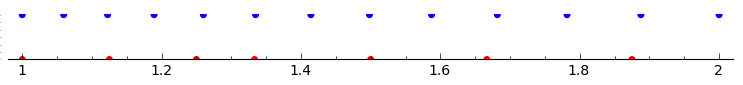
\includegraphics[scale=0.65]{figures/equally_temperedness.png}
    \caption{Blue points represent equally tempered scale and red points represent Ptolemaic scale.}
    \label{equally_temperedness}
\end{figure}

Let us state a formal definition of equally temperedness.

\begin{definition}
    An \emph{equally tempered tonal space} is a cyclic subgroup of $(\R,\cdot)$.
    A subset of such a group is called an \emph{equally tempered scale}.
\end{definition}

Thus we can consider an equally tempered tonal space as being an approximation of a tonal space.
Most of the musical compositions are written using such approximations, instead of an actual tonal space.
This has several practical and historical reasons.
We will not study equally tempered scales further, as it is beyond the scope of this thesis.
However, this notion is needed for understanding the connection between tonal spaces and actual music that is mostly written in equally tempered scale.
In chapter \ref{application} we will need this knowledge, when we want to apply the theory to a musical composition.


\chapter{Distance between Tones}
\label{distance}
There is more to tones than multiplication.
The notions we are studying in this chapter will satisfy the axioms of distance.
Let us recall the notions norm and metric for abelian groups and thus for tonal spaces.

\section{Metric on abelian groups}

\begin{definition}
    Let $G$ be an abelian group.
    Then a function $\|\cdot\|:G \to [0,\infty)$ is called a \emph{norm} on $G$, if it suffices the following properties for all $g,h \in G$.
	\begin{enumerate}[i]
		\item $\|g\| = 0 \Leftrightarrow g=1$
        \item $\|g\| = \|g^{-1}\|$
		\item $\|g \cdot h\| \leq \|g\| + \|h\|$
	\end{enumerate}
\end{definition}

\begin{definition}
	A \emph{metric} on an abelian group $G$ is a function $d:G \times G \to [0,\infty)$, sufficing the following properties for all $g,h,j \in G$:
	\begin{enumerate}[i]
		\item $d(g,h) = 0 \Leftrightarrow g=h$
		\item $d(g,h) = d(h,g)$
		\item $d(g,j) \leq d(g,h) + d(h,j)$
	\end{enumerate}
\end{definition}

A norm defined on an abelian group can induce a metric, as pointed out by the following lemma.

\begin{lemma}
    Let $G$ be an abelian group with a norm.
    Define $d:G \times G \to [0,\infty), (g,h) \mapsto \|gh^{-1}\|$.
    Then $d$ is a metric.
	\label{norm_to_metric}
\end{lemma}
\begin{proof}
	We show that $d$ suffices the properties of a metric.
    \begin{enumerate}[i]
        \item $d(g,h) = 0 \Leftrightarrow \|gh^{-1}\| = 0 \Leftrightarrow gh^{-1} = 1 \Leftrightarrow g = h$.
        \item $d(g,h) = \|gh^{-1}\| = \|(hg^{-1})^{-1}\| = \|hg^{-1}\| = d(h,g)$.
        \item $d(g,j) = \|gj^{-1}\| = \|gh^{-1}hj^{-1}\| \leq \|gh^{-1}\|+ \|hj^{-1}\| = d(g,h) + d(h,j)$.
    \end{enumerate}
	Thus $d$ is a metric on $G$.
\end{proof}

\section{Melodic distance}
Some tones sound higher in pitch than others.
The higher the tone, the higher its sound.
We will refer to this kind of distance as \emph{melodic distance}.
If we want to measure this difference in pitch as a metric, we must decide how we want the metric to behave.

If we informally ``stack'' a musical interval upon a tone, this corresponds to multiplying with a number.
For instance if we ``add'' an ``octave'' to a tone, this corresponds to multiplying the tone with $2$.
This suggests that we might want to turn multiplication into addition, when converting ratio between tones to distance in pitch.
Namely, the notion of ``adding'' an octave to a tone is very intuitive.
To turn multiplication into addition, we need an injective group homomorphism between $\Q$ and $(\mathbb{R},+)$.
This then can induce a norm, as pointed out by the following lemma.

\begin{lemma}
    Let $G$ be an abelian group, and $\varphi : G \to (\mathbb{R},+)$ an injective group homomorphism.
    Then $\| \cdot \| : G \to \mathbb{R}_{\geq 0}, g \mapsto |\varphi(g)|$ a norm, where $| \cdot |$ is the norm that takes numbers to their absolute value.
    \label{homomorphism_to_metric}
\end{lemma}
\begin{proof}
    We show that the properties of a norm are fulfilled.
    \begin{enumerate}[i]
        \item $\|g\| = 0 \Leftrightarrow \varphi(g) = 0 \Leftrightarrow g = 1$
        \item $\|g^{-1}\| = |\varphi(g^{-1})| = |-\varphi(g)| = |\varphi(g)| = \|g\|$
        \item $\|gh\| = |\varphi(gh)| = |\varphi(g) + \varphi(h)| \leq |\varphi(g)| + |\varphi(h)| = \|g\| + \|h\|$
    \end{enumerate}
\end{proof}

For a norm to actually measure difference in pitch, an additional property is needed.
Namely, we need to be sure that if a tone $t$ is strictly further away from the tonic than a tone $s$, then $\|s\| < \|t\|$.
The following definition of melodic distance will suffice this property, as shown in theorem \ref{order_preserving_homomorphism}.

\begin{definition}
    Let $T$ be a tonal space and $\varphi : T \to (\mathbb{R},+)$ an injective group homomorphism,
    with the property that $s \leq t \Leftrightarrow \varphi(s) \leq \varphi(t)$, for all $s,t \in T$.
    Then the norm that follows by applying lemma \ref{homomorphism_to_metric}, is called a \emph{melodic norm}.
    The metric that can be induced from this norm by lemma \ref{norm_to_metric}, is called a \emph{melodic distance}.
\end{definition}

\begin{theorem}
    \label{order_preserving_homomorphism}
    Let $T$ be a tonal space and $\varphi : T \to (\mathbb{R},+)$ inducing a melodic norm $\| \cdot \|$ on $T$.
    Then $ \max(s,s^{-1}) < \max(t,t^{-1}) \Leftrightarrow \|s\|<\|t\|$.
    In other words, a tone $t$ is strictly further away from the tonic than a tone $s$, if and only if $\|s\| < \|t\|$.
\end{theorem}
\begin{proof}
    Denote $s' = \max(s,s^{-1})$ and $t' = \max(t,t^{-1})$.
    Notice that $1 \leq s'$ and $1 \leq t'$.
    Suppose $s' < t'$.
    We know that $s \leq t \Leftrightarrow \varphi(s) \leq \varphi(t)$, for all $s,t \in T$.
    So 
    \begin{alignat*}{3}
        & 1 & &\leq s'             & &<  t' \\
        & 0 & &\leq \varphi(s')    & &<  \varphi(t') \\
        & 0 & &\leq |\varphi(s')|  & &<  |\varphi(t')| \\
        & 0 & &\leq \|s\|          & &<  \|t\|
    \end{alignat*}
    
    Now suppose $\|s\|<\|t\|$.
    Then 
    \begin{alignat*}{3}
        & 0 & &\leq \|s\|          & &<  \|t\| \\
        & 0 & &\leq |\varphi(s')|  & &<  |\varphi(t')| \\
        & 0 & &\leq \varphi(s')    & &<  \varphi(t') \\
        & 1 & &\leq s'             & &<  t' 
    \end{alignat*}
\end{proof}

\begin{example}
    \label{log_as_melodic_distance}
    Let $T$ be a tonal space and $s,t \in T$.
    Any logarithm is an injective group homomorphism from $T$ to $(\mathbb{R},+)$, since $\log(st) = \log(s) + \log(t)$, no matter what the base of the logarithm is.
    Notice that $s \leq t \Leftrightarrow \log(s) \leq \log(t)$, so $t \mapsto |\log(t)|$ is a melodic norm and $(s,t) \mapsto |\log(s)-\log(t)|$ a melodic distance.
\end{example}

\section{Harmonic distance}
There is a second kind of distance between tones.
Some pairs of tones sound more ``consonant'' when played together than others.
This too can be interpreted as distance in the sense that the further some tone is away from another tone, the more ``dissonant'' their combination will sound.
We will refer this kind of metric \emph{harmonic distance}.

Remember that Pythagoras discovered how easy ratio's are related to ``consonant'' sounds.
Notice that the ratio between two tones is the tone the first tone has to be multiplied with to obtain the second tone.
Namely, if we multiply a tone $t$ with the tone $\frac{s}{t}$, we get $t \cdot \frac{s}{t} = s$.
So formally speaking, ``simple'' tones are related to ``consonant'' sounds, according to Pythagoras.
%The more ``simple'' a ratio between two tones is, the more ``consonant'' the sound.
If we then want to determine the harmonic distance between two tones, we need to judge their ratio on ``simpleness''.
%We can deduce from this that we can construct tones that are very close to the tonic by multiplying the tonic with ``simple'' numbers.
This raises the question, which tones are ``simple''?
%Or more specifically, how can we determine the ``simpleness'' from numbers?
If we first find a formula for the simpleness of tones, we can use it as a norm.
This norm will then induce a metric by lemma \ref{norm_to_metric}.
So essentially we are looking for an harmonic norm $\| \cdot \| : \Q \to \mathbb{R}_{\geq 0}$, which reflects ``simpleness'' of tones.
We will state some assumptions we make about the harmonic distance and then formulate a formal definition.

First, we have to make an assumption about products of tones.
We want that if we multiply a tone $t \in \mathbb{N}$ with another tone $s \in \mathbb{N}$, that $\|st\| = \|s\|+\|t\|$.
This makes sense, since both $t$ and $s$ have some degree of simpleness, and therefore their product has both degrees of simpleness in it, suggesting that the resulting simpleness should be the sum of the parts.
Now if $t$ and $s$ are not natural, some problem may occur.
For example, $t$ may be the inverse of $s$.
In that case, we definitely don't want that $\|st\| = \|s\|+\|t\|$, since $\|st\|=\|t^{-1}t\|=\|1\|$, which is very, very simple.
Generally speaking, if $t = a \cdot b$ is a tone with $a$ and $b$ such that the numerator of $a$ is coprime with the denominator of $b$ and vice versa, we want that the value of $t$ is the same as the values of $a$ and $b$ added together.
Remember that two numbers being coprime means that the greatest common divisor between those two numbers is $1$.

The second assumption we make, is that any tone $t$ is just as simple as its inverse $t^{-1}$.
This also makes sense, since we decided to study relative harmony only, meaning that we wouldn't care about actual number values of tones, but only about their ratio to the tonic. 
That implies that we assume that tones behave the same under translation.
So, considering the harmonic distance between $1$ and $t$, we could translate both $1$ and $t$ down by $t$, resulting in $t^{-1}$ and $1$.
Now if tones behave the same under translation, clearly the harmonic distance between $1$ and $t$ and between $t^{-1}$ and $1$ should be the same, implying that $\|t\| = \|t^{-1}\|$.

The third and last assumption we have to make, is that $1$ is the only tone with norm $0$.
This makes sense because the harmonic distance between two tones should indeed be zero if and only if they are the same.

Let us list the assumption we just stated as axioms for the harmonic norm.
\begin{definition}
    A \emph{harmonic norm} $\| \cdot \|$ is a norm on $\Q$ sufficing the following properties.
    \begin{enumerate}[i]
        \item If $t = a \cdot b$ is a tone with $a$ and $b$ such that the numerator of $a$ is coprime with the denominator of $b$ and vice versa, then $\|t\| = \|a\|+\|b\|$.
        \item For any tone $t$, $\|t\| = \|t^{-1}\|$.
        \item For any tone $t$, $\|t\| = 0 \Leftrightarrow t = 1$.
    \end{enumerate}
    The metric that can be induced from this norm by lemma \ref{norm_to_metric}, is called a \emph{harmonic distance}.
\end{definition}

Let us verify that the notion of harmonic norm we just defined satisfies the axioms of a norm.

\begin{lemma}
    A harmonic norm $\| \cdot \|$ is indeed a norm.
\end{lemma}
\begin{proof}
    We show that $\| \cdot \|$ suffices the properties of a norm.
    \begin{enumerate}[i]
        \item $\|t\| = 0 \Leftrightarrow t = 1$ (by definition)
        \item $\|t^{-1}\| = \|t\|$ (by definition)
        \item Let $t = \frac{ax}{by},s = \frac{cy}{dx}$ two tones such that $ax$ is coprime with $by$, $cy$ is coprime with $dx$, $a$ is coprime with $d$ and $b$ is coprime with $c$.
            Note that any two tones can be written this way. 
            Now 
    \begin{eqnarray*}
            \|ts\| &=& \|\frac{ax}{by} \frac{cy}{dx}\|  \\
            &=& \|\frac{a}{b} \frac{c}{d}\| \\
            &=& \|\frac{a}{b}\| + \|\frac{c}{d}\|  \\
            &\leq& \|\frac{a}{b}\| + \|\frac{x}{y}\| + \|\frac{c}{d}\| + \|\frac{y}{x}\|  \\
            &=& \|\frac{a}{b}\frac{x}{y}\| + \|\frac{c}{d}\frac{y}{x}\|  \\
            &=& \|t\| + \|s\|.
    \end{eqnarray*}
    \end{enumerate}
\end{proof}

It appears that we only need to assign values of ``simpleness'' to each generator of a tonal space.
Then the ``simpleness'' of every other tone can be determined from this, as pointed out by theorem \ref{function_to_harmonic_norm}.
Thus a function assigning strictly positive numbers to generators of a tonal space, induces a harmonic metric.

\begin{theorem}
    Let $T$ be a tonal space and $\| \cdot \|$ a harmonic norm on $T$.
    Then $\|t\| = \varphi(p_0) + \dots + \varphi(p_n) + \varphi(q_0) + \dots + \varphi(q_m)$, where $\varphi$ is a function that assigns a strictly positive number to every prime generator of $T$.
    \label{function_to_harmonic_norm}
\end{theorem}
\begin{proof}
    Let $T$ be a tonal space and $\| \cdot \|$ a harmonic norm on $T$.
    Let $\varphi$ such that $\varphi(p) = \|p\|$ for all prime generators of $T$.
    Now let $t \in T$ with unique prime factorization $\frac{p_0 \dots p_n}{q_0 \dots q_m}$.
    Then 
    \begin{eqnarray*}
        \|t\| &=& \|\frac{p_0 \dots p_n}{q_0 \dots q_m}\| \\
            &=& \|p_0 \dots p_nq_0^{-1} \dots q_m^{-1}\| \\
            &=& \|p_0\|+ \dots + \|p_n\| + \|q_0^{-1}\| + \dots + \|q_m^{-1}\| \\
            &=& \|p_0\|+ \dots + \|p_n\| + \|q_0^{-1}\| + \dots + \|q_m^{-1}\| \\
            &=& \|p_0\|+ \dots + \|p_n\| + \|q_0\| + \dots + \|q_m\|\\
            &=& \varphi(p_0) + \dots + \varphi(p_n) + \varphi(q_0) + \dots + \varphi(q_m)
    \end{eqnarray*}
\end{proof}


\begin{example}
    \label{eulers_formula}
    Let $T = \gen{2,3,5}$ be a tonal space.
    Define a harmonic norm such that $\|2\| = 1$, $\|3\| = 2$ and $\|5\| = 4$.
    By theorem \ref{function_to_harmonic_norm}, this indeed induces a harmonic norm.
    Again by by lemma \ref{norm_to_metric} this induces a harmonic distance.
\end{example}

\begin{remark}
    In his work \emph{Tentamen novae theoriae musicae ex certissismis harmoniae principiis dilucide expositae} Leonhard Euler studied music theory. 
    He came up with a formula attempting to measure the amount of what he called ``agreeableness'' which can be found in a set of tones played together. \cite{Euler}
    This comes close to what we would call the amount of ``consonance''.
    His formula is very similar to the harmonic distance in example \ref{eulers_formula}, but there are a few differences.
    First of all, he liked to add $1$ to the formula, implying that that amount of consonance of $1$ (the tonic) is $1$.
    This causes his formula not to be compatible with the axioms of distance.
    Secondly, he did not consider fractional tones, since any set of fractional tones can be made integer by scaling them up.
    Apart from that, the formula is the same.
    For every prime $p$, he assigned the value $p-1$ as agreeableness, just like we did in example \ref{eulers_formula}.
    However, he did not formulate any assumptions and gave no proof for his formula.
\end{remark}


\section{Melodic-Harmonic distance}
Nothing keeps us from combining melodic metric and harmonic metric into a new metric.

\begin{theorem}
    The sum of two norms, is again a norm.
    \label{sum_of_norms}
\end{theorem}
\begin{proof}
    Let $\|\cdot\|_1$ and $\|\cdot\|_2$ be two norms on an abelian group $G$.
    Define $\|\cdot\| = \|\cdot\|_1 + \|\cdot\|_2$.
    We prove the properties of a norm.
    \begin{enumerate}[i]
        \item $\|g\| = \|g\|_1 + \|g\|_2 = 0 \Leftrightarrow \|g\|_1 = 0 $ and $\|g\|_2 = 0 \Leftrightarrow g = 1$
        \item $\|g^{-1}\| = \|g^{-1}\|_1 + \|g^{-1}\|_2 = \|g\|_1 + \|g\|_2 = \|g\|$
        \item $\|gh\| = \|gh\|_1 + \|gh\|_2 \leq  \|g\|_1 + \|g\|_2 + \|h\|_1 + \|h\|_2 = \|g\| + \|h\|$
    \end{enumerate}
\end{proof}

\begin{corollary}
    The sum of a melodic metric and a harmonic metric is again a metric
    \label{sum_of_metrics}
\end{corollary}
\begin{proof}
    Write the melodic metric and the harmonic metric as norms and apply theorem \ref{sum_of_norms}.
    Then applying lemma \ref{norm_to_metric} yields the result.
\end{proof}

\begin{example}
    Let $T = \gen{2,3,5}$ be a tonal space.
    Define a harmonic norm such that $\|2\|_H = 1$, $\|3\|_H = 2$ and $\|5\|_H = 4$.
    Define the melodic norm such that $\|t\|_M = \log(t)$, for every $t\in T$.
    Then \[\|t\|_M + \|t\|_H = \log(t) + \sum_{p \text{ prime factor of } t}{(p-1)}\] is a norm.
\end{example}

\chapter{Applying the Theory}
\label{application}
We will look at an application of the theory to a small part of a musical composition.
The musical piece we choose is Pachelbel's Canon, the canon written by the German Baroque composer, Johann Pachelbel, taken from his \emph{Canon and Gigue for 3 violins and basso continuo}.
This is a famous piece and suitable for studying basic music theory, since the theme is very common in western music and there are not too many voices.

\section{Recovering approximation}
The first problem we encounter is that the piece is written in equally tempered scale.
Remember from section \ref{section_equally_temperedness} that this means that we do not know the actual tones used in the piece, but rather approximations of these tones.
We will first have to convert these approximations to tones before we can study them like we did in the previous chapters.
For now we will not study approximation recovery algorithms, but use an easy method to derive the actual tones that are used in the composition.
For each equally tempered tone, we will just take the closest tone occuring in the Ptolemaic Sequence, presented in example \ref{ptolemaic_sequence}.
Since this piece is written in major scale and contains no ``accidentals'', this will do.
We will choose the note ``d'' as the tonic, since this piece is written in ``D major''.
This choice is crucial, since it greatly affects the resulting tones.

\section{Metrical analysis of a monophonic part}
Let us study the first six measures played by the first violin. The partiture of this piece in traditional notation, along with the resulting tones are displayed in figure \ref{fig_first_violin_tones}.

\begin{figure}[H]
    \centering
    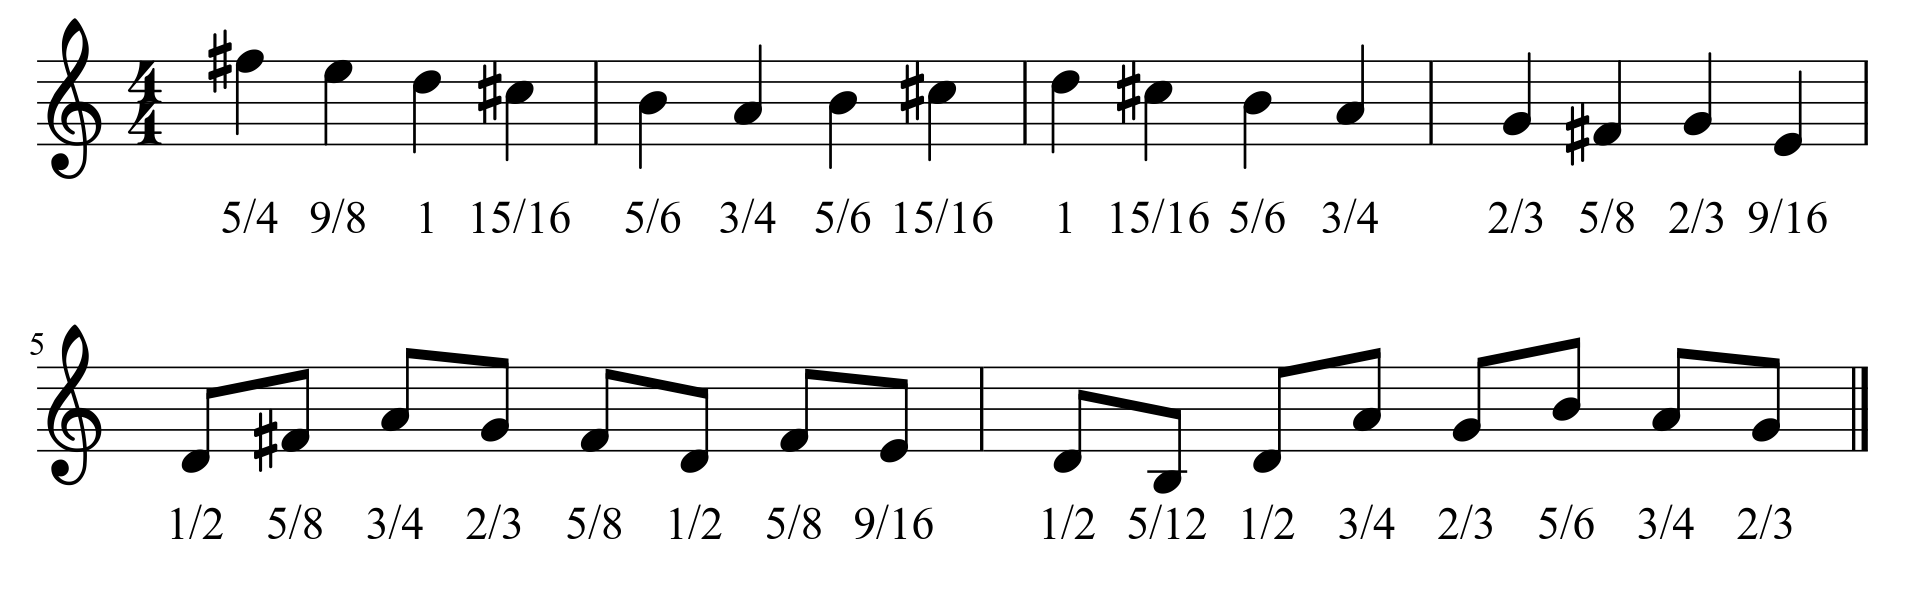
\includegraphics[scale=0.25]{figures/fig_first_violin_tones.png}
    \caption{First six measures of first violin, showing corresponding numbers}
    \label{fig_first_violin_tones}
\end{figure}

Let us now apply the tools we developed in chapter \ref{distance}.
We first want to compute the melodic distance between every tone and its subsequent tone.
This will then point out how the melody jumps up and down.
We are free to choose the formula $\log_{2^{\frac{1}{12}}}(t)$ as melodic distance, by example \ref{log_as_melodic_distance}.
To make the numbers nice, we round the melodic distances.
Unsurprisingly, this rounded melodic distance exactly corresponds with the number of tones in the twelve tone equally tempered scale (informally known as semitones) between the two subsequent tones.
The results are displayed in figure \ref{fig_first_violin_melodic_distance}.
One should interpret the number below a tone as the melodic distance that had to be travelled from the previous tone, to arrive at the current tone.

\begin{figure}[H]
    \centering
    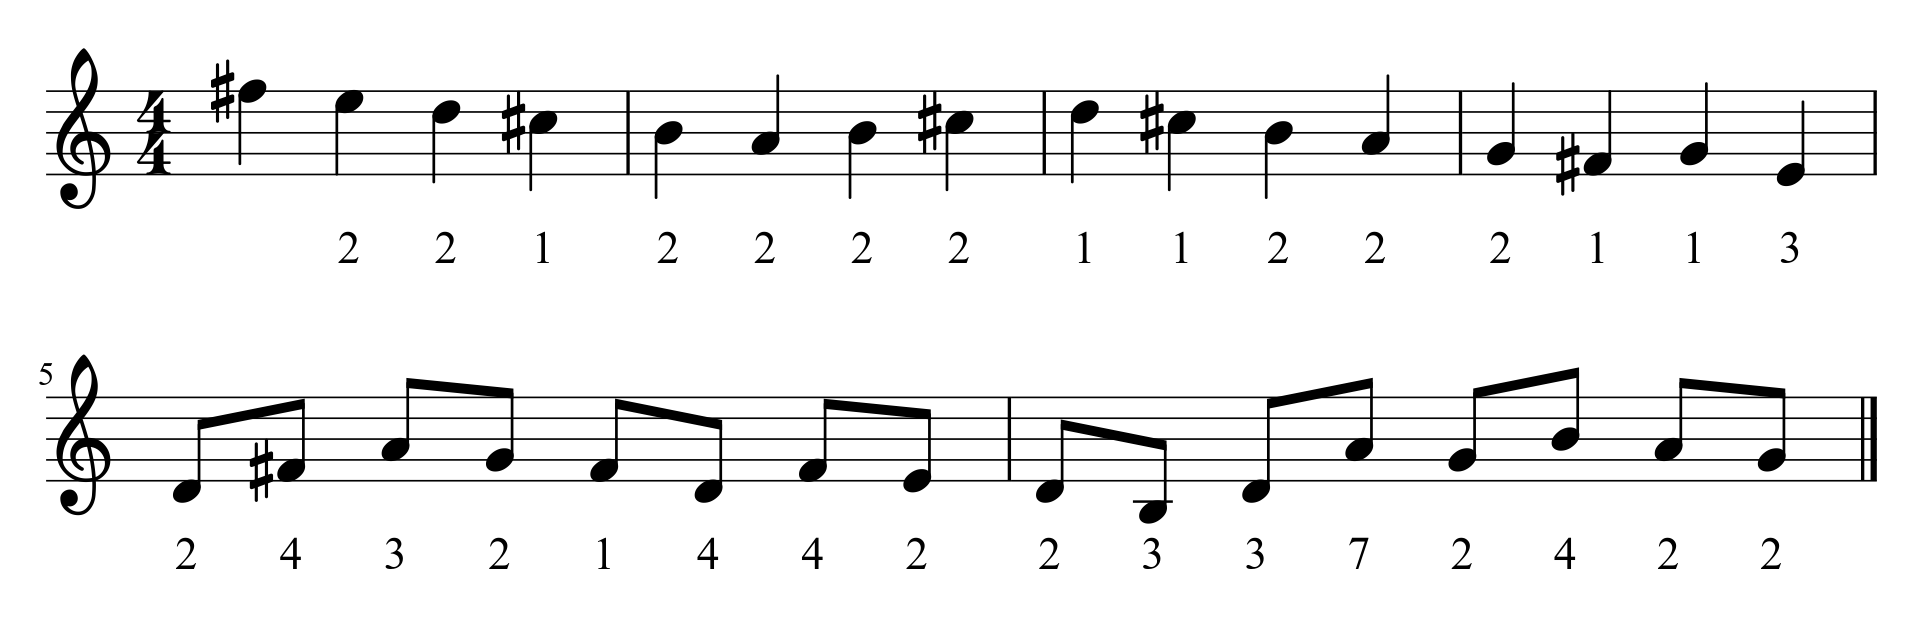
\includegraphics[scale=0.25]{figures/fig_first_violin_melodic_distance.png}
    \caption{First six measures of first violin, showing rounded melodic distance to the previous tone}
    \label{fig_first_violin_melodic_distance}
\end{figure}

The same way, we can compute the harmonic distance between subsequent tones.
We decide to use the formula from example \ref{eulers_formula}.
The results are displayed in figure \ref{fig_first_violin_harmonic_distance}.
The number right below a tone, is the harmonic distance between that tone and the previous tone.
In other words, it represents the harmonic distance that had to be travelled to arrive from the previous tone at the current tone.

\begin{figure}[H]
    \centering
    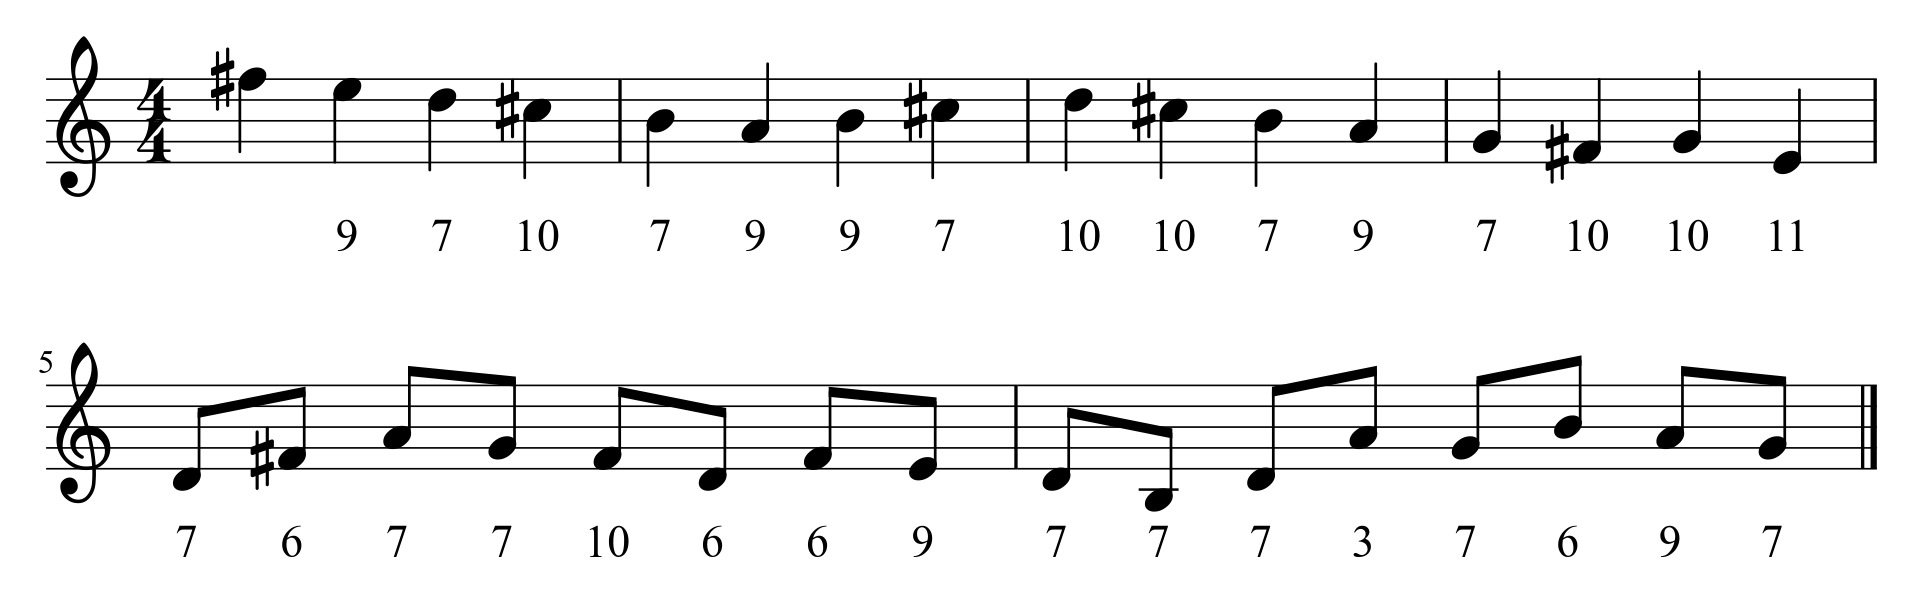
\includegraphics[scale=0.25]{figures/fig_first_violin_harmonic_distance.png}
    \caption{First six measures of first violin, showing harmonic distance to the previous tone}
    \label{fig_first_violin_harmonic_distance}
\end{figure}

Analyzing figures \ref{fig_first_violin_harmonic_distance} and \ref{fig_first_violin_melodic_distance}, we can make a few interesting observations.
First of all, it appears that most of the time, when the harmonic distance is relatively high, the melodic distance is relatively low, and vice versa.
To confirm this, we like to display the melodic-harmonic distance, as a sum of the two previous distances.
By corollary \ref{sum_of_metrics} this is indeed a metric.
This then results in figure \ref{fig_first_violin_melodic_harmonic_distance}.
Indeed, the spread appears to be small, suggesting that melodic distance and harmonic distance neutralize each other.

\begin{figure}[H]
    \centering
    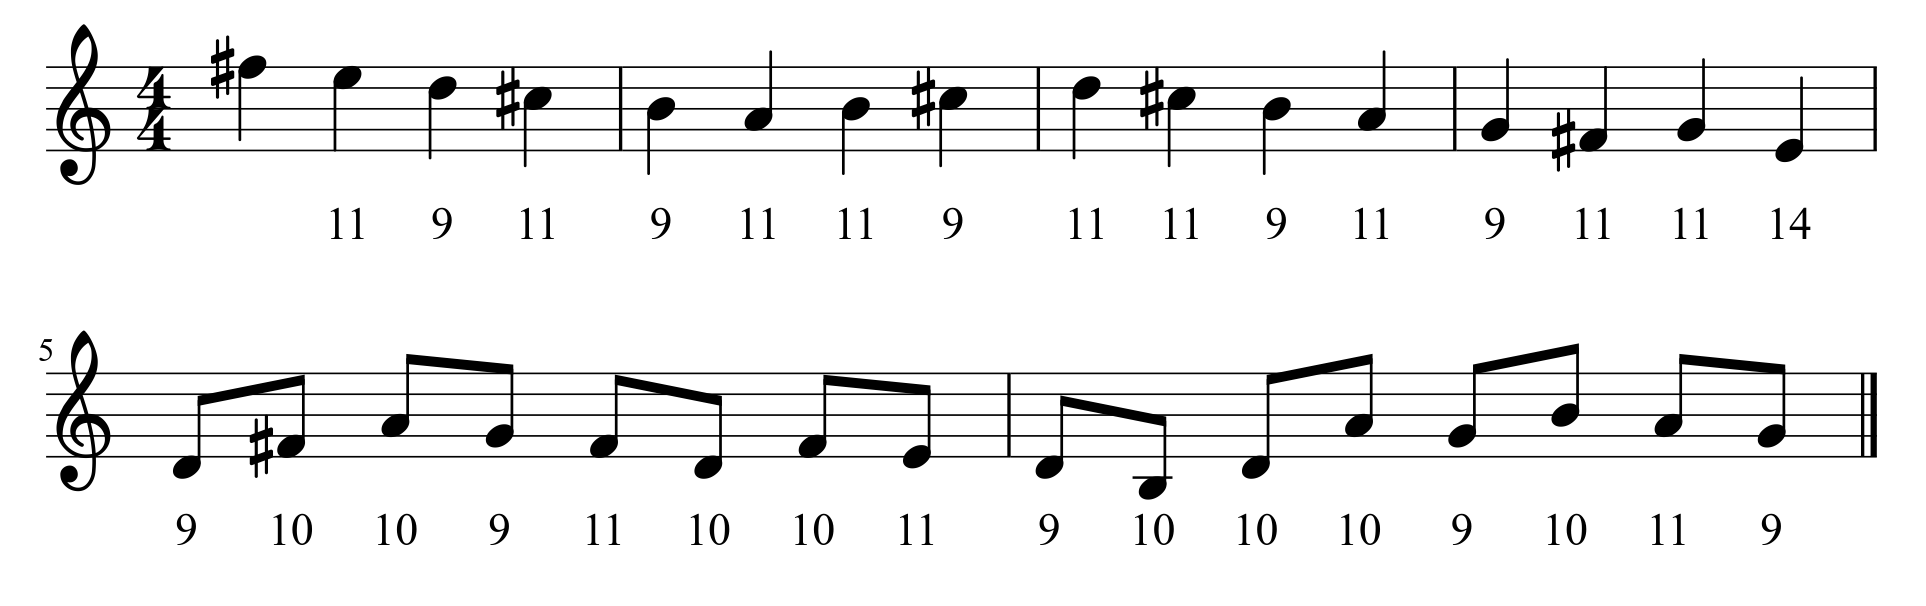
\includegraphics[scale=0.25]{figures/fig_first_violin_melodic_harmonic_distance.png}
    \caption{First six measures of first violin, showing melodic-harmonic distance to the previous tone}
    \label{fig_first_violin_melodic_harmonic_distance}
\end{figure}

It may also be interesting to display the harmonic distance between every tone and the tonic.
Remember that in this piece the note which is informally referred to as ``d'' corresponds with $1$, and is therefore called tonic.
See figure \ref{fig_first_violin_tones}.
We can then compare this with the distance between subsequent tones.
For convenience we place the harmonic distance to the previous tone above, and the harmonic distance to the tonic below.
The results are displayed in figure \ref{fig_first_violin_harmonic_distance_to_tonic}.

\begin{figure}[H]
    \centering
    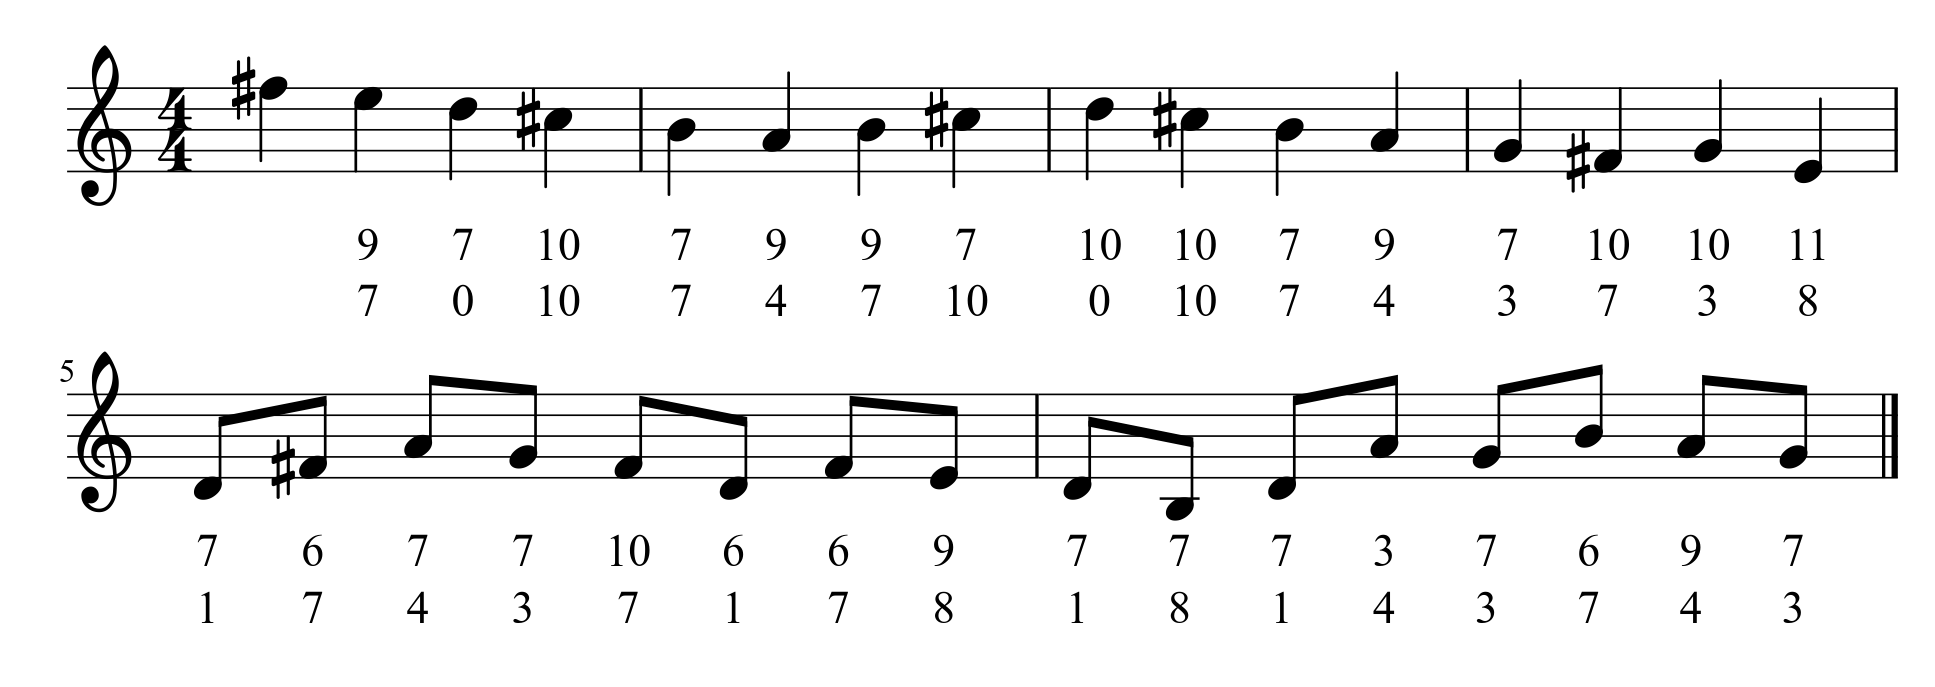
\includegraphics[scale=0.25]{figures/fig_first_violin_harmonic_distance_to_tonic.png}
    \caption{First six measures of first violin, showing harmonic distance to previous tone above and harmonic distance to tonic below.}
    \label{fig_first_violin_harmonic_distance_to_tonic}
\end{figure}

We can observe that the distance to the previous tone is most of the time greater than the distance to the tonic.
There are three exceptions, where the distance to the tonic is $7$ and the distance to the previous tone is $6$.
Perhaps these exeptions could serve as a starting point for formalization of other concepts, like functions of harmony, or resolution, but that is beyond the scope of this thesis.
Apart from these exceptions, the observation holds.

\section{Metrical analysis of a two-voice polyphonic part}
Let us not stick to the first six measures of the first violin, but consider another part.
We would like to analyze polyphony now.
Since we didn't say anything about rythm and related things, we will restrict ourselves to a part where tones are played simultanuously.
We therefore decide to consider measures 11 till 15 of both the first and the second violin.
The tones are displayed in figure \ref{fig_first_second_violin_tones}.

\begin{figure}[H]
    \centering
    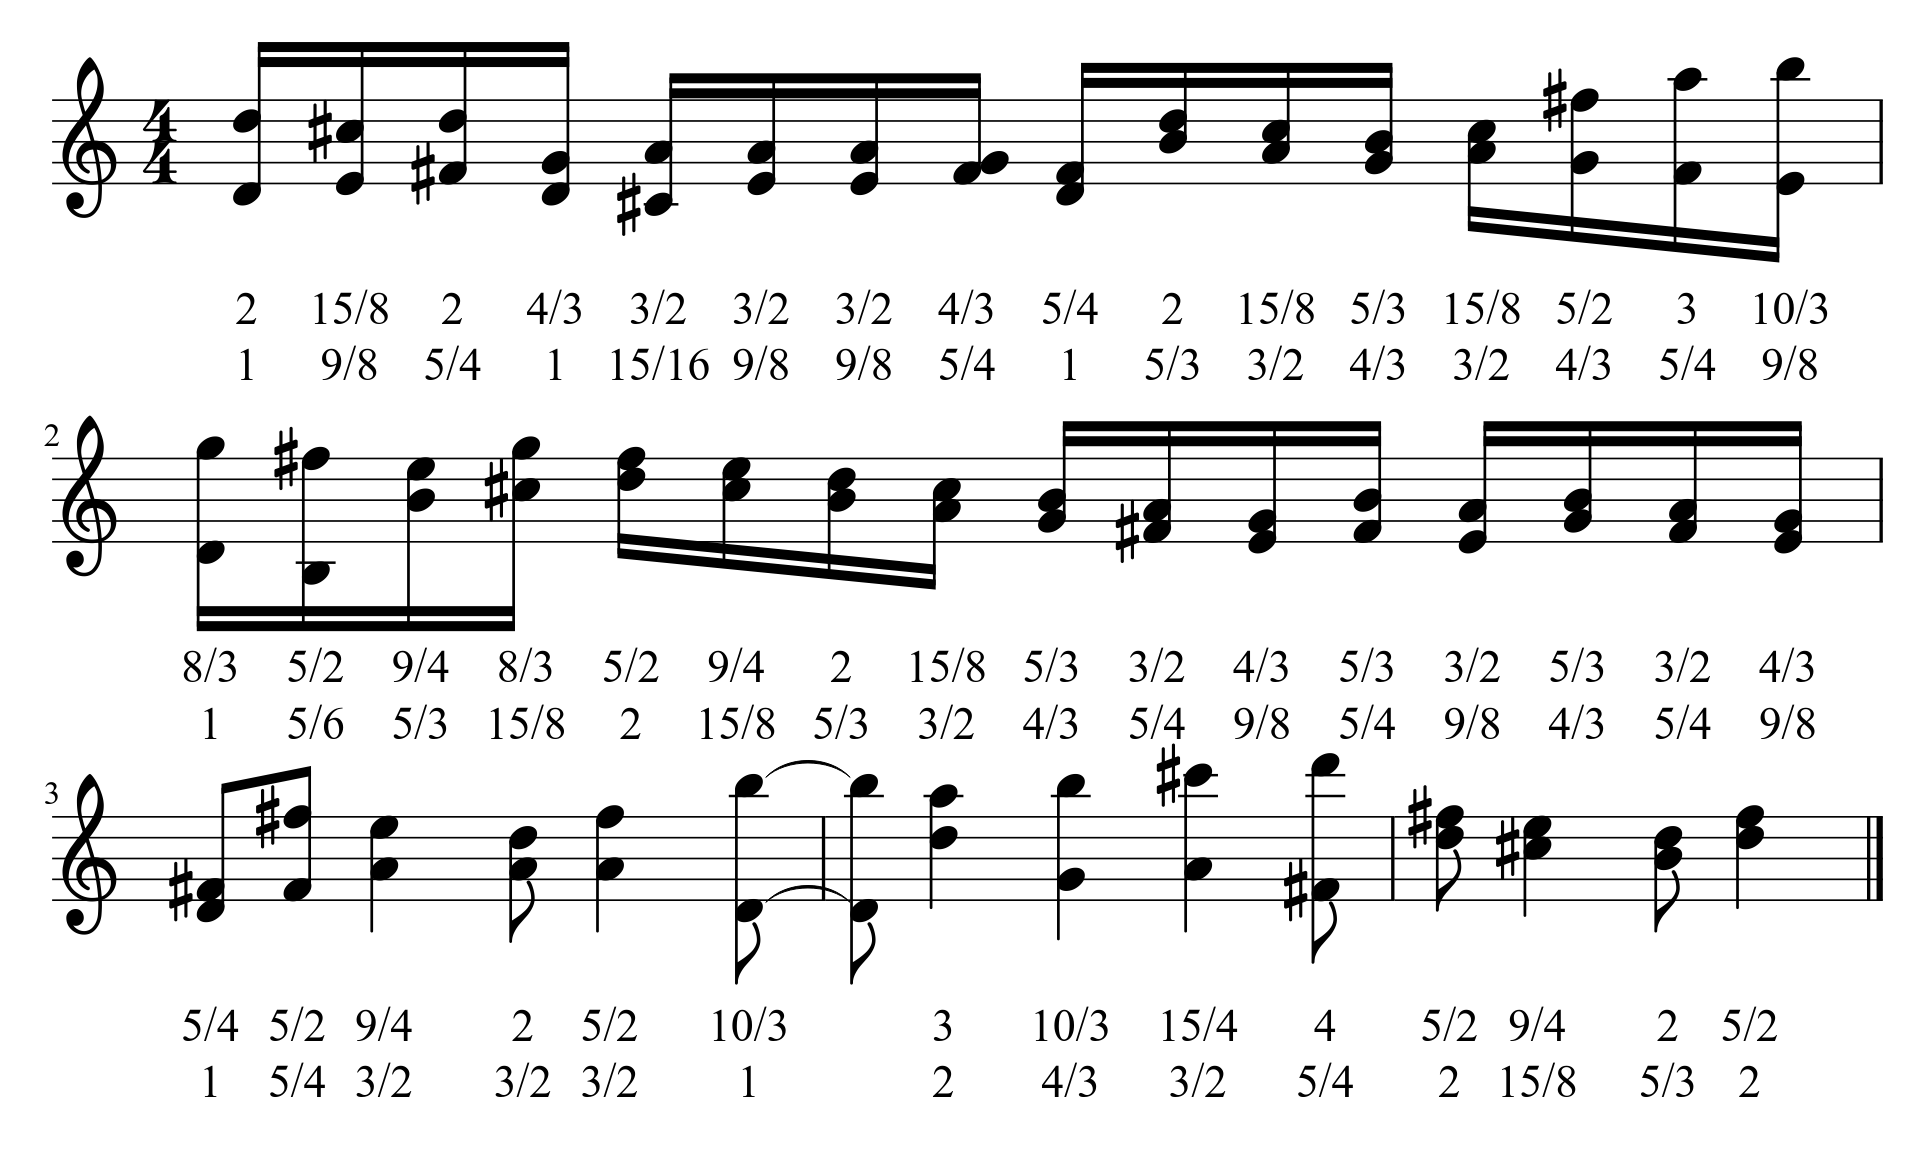
\includegraphics[scale=0.25]{figures/fig_first_second_violin_tones.png}
    \caption{Measures 11 till 15 of first and second violin, showing corresponding numbers}
    \label{fig_first_second_violin_tones}
\end{figure}

We can now compute the harmonic distance and the melodic distance between each pair of tones that are played simultanuously.
The result is displayed in figure \ref{fig_first_second_violin_melodic_and_harmonic_distance_self}.

\begin{figure}[H]
    \centering
    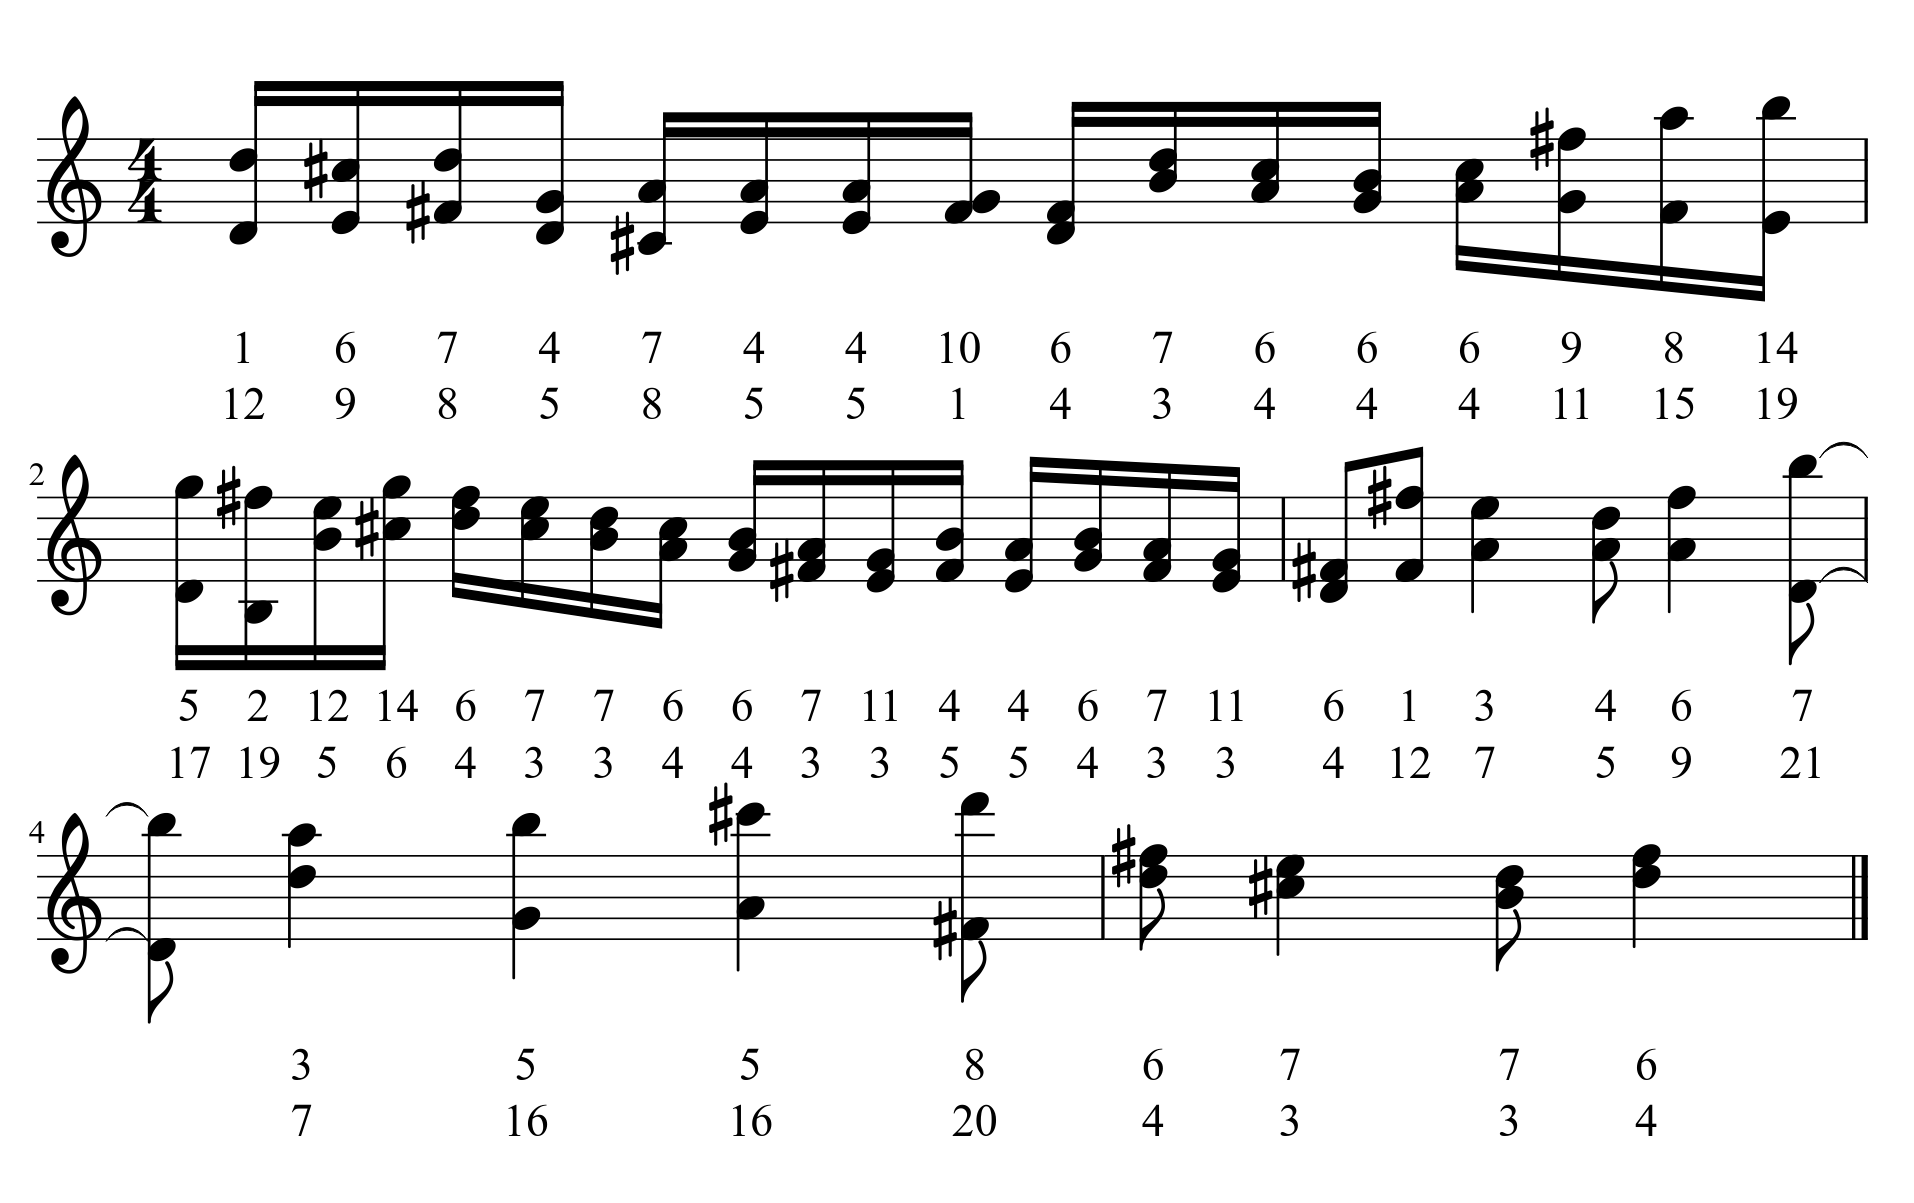
\includegraphics[scale=0.25]{figures/fig_first_second_violin_melodic_and_harmonic_distance_self.png}
    \caption{Measures 11 till 15 of first and second violin, showing harmonic distance above and melodic distance below between tones played simultanuously}
    \label{fig_first_second_violin_melodic_and_harmonic_distance_self}
\end{figure}

One might wonder if the melodic distance and the harmonic distance neutralize each other for tones that are played simultanuously.
To check this, we compute the melodic-harmonic distance, as before.
The result is displayed in figure \ref{fig_first_second_violin_melodic_harmonic_distance_self}.

\begin{figure}[H]
    \centering
    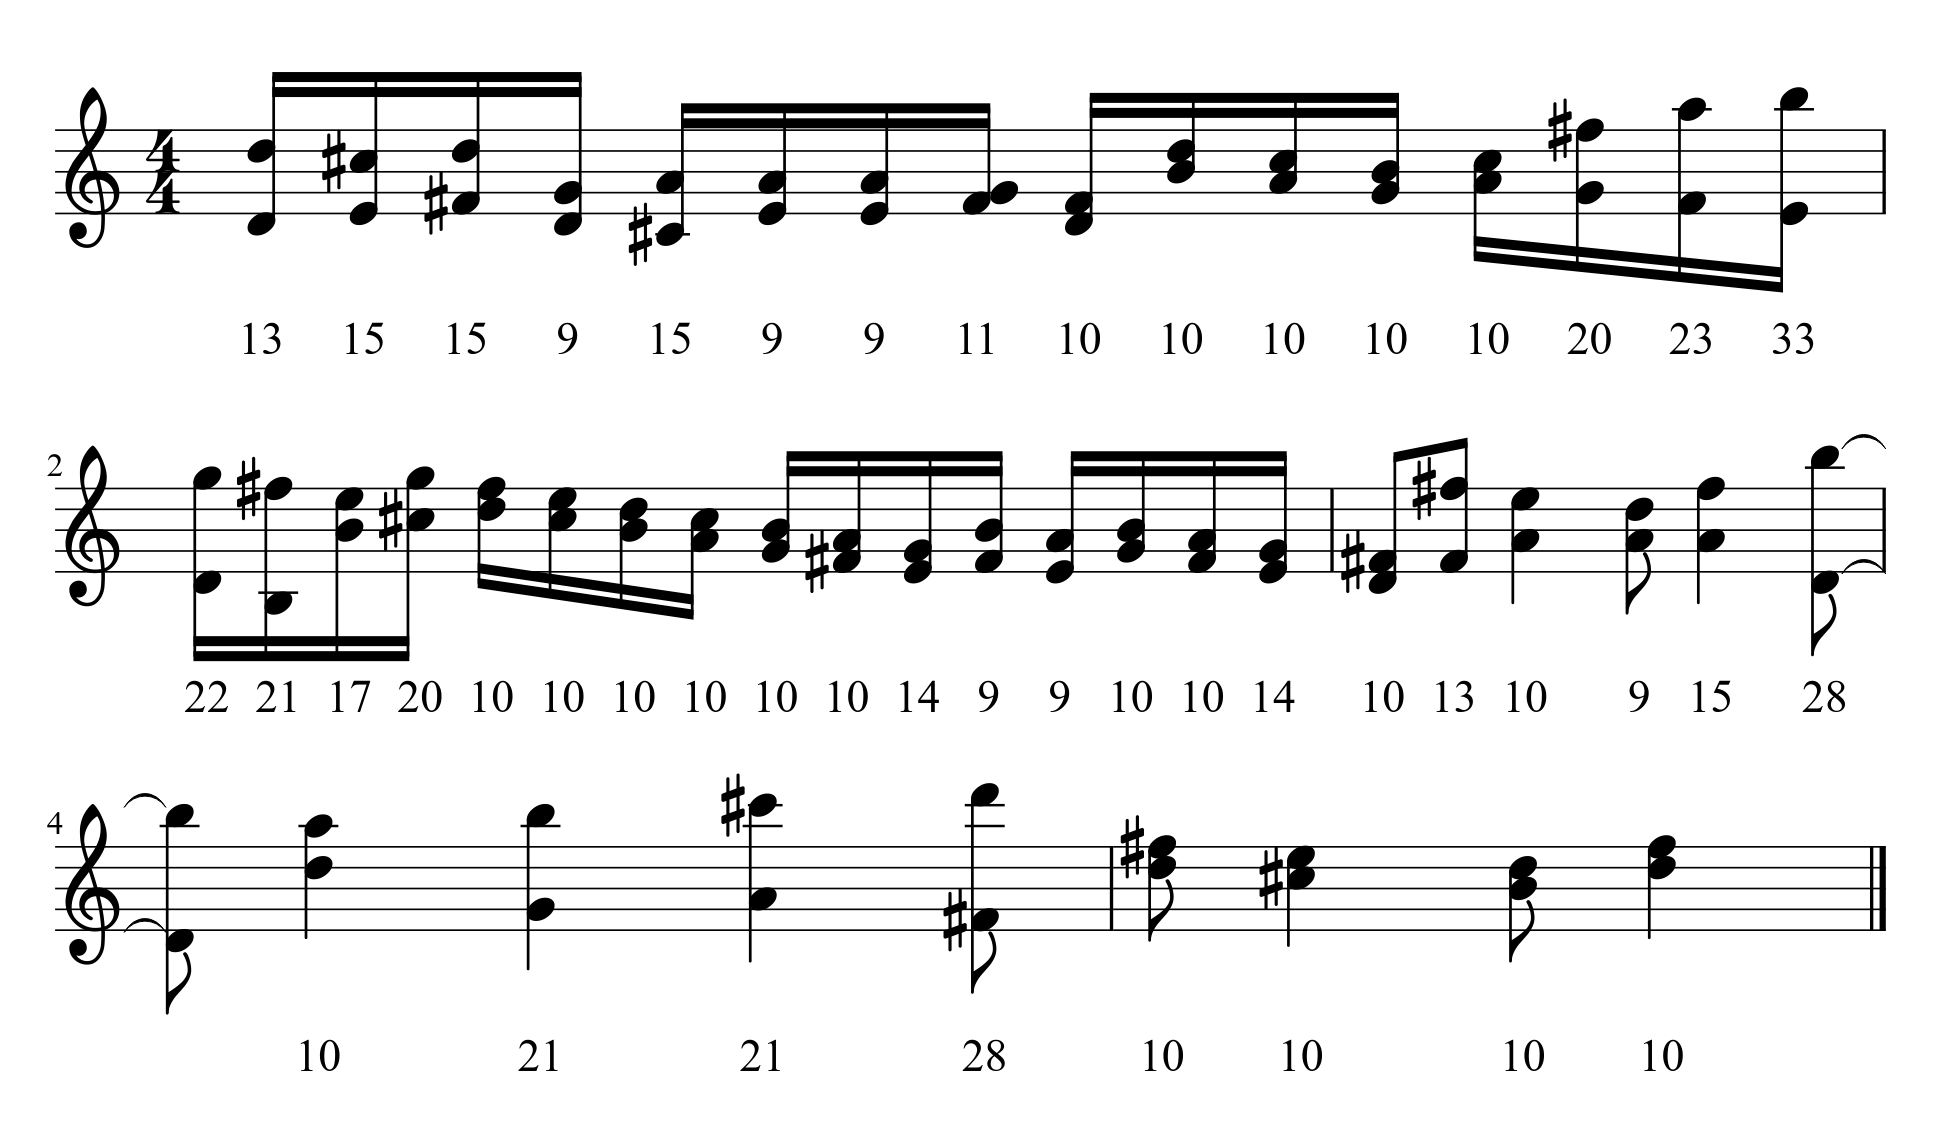
\includegraphics[scale=0.25]{figures/fig_first_second_violin_melodic_harmonic_distance_self.png}
    \caption{Measures 11 till 15 of first and second violin, showing melodic-harmonic distance between tones played simultanuously}
    \label{fig_first_second_violin_melodic_harmonic_distance_self}
\end{figure}

As we can see, this does not hold.
The numbers are very scattered, suggesting that melodic distance and harmonic distance do not behave adversely for simultanuously played tones.
However, it is noteworthy that there are relatively large sequences of $10$'s co\"inciding with the two voices going up and down simultanuously and having a difference of exactly two tones in the Ptolemaic scale.
An exception on this is the pair of tones $\frac{9}{8}$ (``e'') and $\frac{9}{8}$ (``g'') having melodic-harmonic distance of $14$ and ocurring twice.
So apparently, melodic and harmonic distance \emph{do} behave adversely in most of the cases where two voices are going up and down simultanuously and are having a difference of exactly two tones in the Ptolemaic scale.


Let us conclude with the remark that the notions of distance we introduced in chapter \ref{distance} do seem to have some meaning, since the results are not completely random.

\chapter*{Epilogue}
As explained in the preface, our goal was not to describe music theory, but rather to think up a formal mathematical theory, which would appear to be at least a little consistent with our experience of music.
In chapter \ref{tonal_space} we tried to formulate what we would consider to be a tone.
This appeared to be a number, in the context of an abelian group under multiplication.
In chapter \ref{distance} we considered several musical phenomena as being a notion of distance.
We gave formal definitions of them, and gave proofs, among others, that they indeed satisfy the axioms of distance.
Finally, in chapter \ref{application}, we applied the theory to a small part of Pachelbells Canon.
Investigating the results, it appeared that there was some consistence in it.
The results were not random, suggesting that the definitions have some meaning outside the formal theory.

Looking back, we can ascertain that we succeeded in formulating a formal mathematical theory about music.
In addition to that, we can partly ascertain that there is some meaning in it, which makes this thesis to have succeeded in its purpose.

%\section{Facts}
%We compute a few properties of Pachelbell's Canon regarding distance.
%Average harmonic/melodic distance. Maximal harmonic/melodic distance.

\begin{thebibliography}{9}

    \bibitem{NeilBibby}
        Neil Bibby
        \emph{Music and Mathematics, Chapter 1}.
        Oxford university press,
        2003.

    \bibitem{CharlesTaylor}
        Charles Taylor
        \emph{Music and Mathematics, Chapter 3}.
        Oxford university press,
        2003.

    \bibitem{DavidFowler}
        David Fowler
        \emph{Music and Mathematics, Chapter 5}.
        Oxford university press,
        2003.

%    \bibitem{MusicandMathematics}
%        Ludger Hofmann-Engl,
%        \emph{Music and Mathematics}.
%        December 2009.

    \bibitem{Euler}
        Charles Samuel Smith,
        \emph{Leonhard Euler's Tentamen Novae Theoriae Musicae: A translation and commentary}.
        Indiana university,
        June 1960.

\end{thebibliography}

\end{document}
